\documentclass{./llncs2e/llncs}
% \usepackage[printonlyused]{acronym} 
\usepackage{graphicx}
\usepackage{fixltx2e}
% 
% Title 
% 

\begin{document}
\title{Human's Cloud}
\titlerunning{Human's Cloud}
\toctitle{Human's Cloud}

\subtitle{A community cloud served by a P2P overlay network on top of the web platform}
\author{David Dias, david.dias@computer.org}
\authorrunning{David Dias}
\tocauthor{David Dias}
\institute{Lisbon Tech, University of Lisbon}

\maketitle


% ^^^^^^^^^^^^^^^^^^^^^^^^^^^^^^^^^^^^^^^^^^^^^^^^^^^^^^^^^^^^^^
% ~~~~~~~~~~~~~~~~~~~~~~~~~~~~~~~~~~~~~~~~~~~~~~~~~~~~~~~~~~~~~~
% ______________________________________________________________

% 
% Abstract 
% 

\begin{abstract}
Grid computing has been around from the 90\'s
No one true way of easy sharing resources
Voluntary computing only used for Research, not accessible for application developers
MOAR

\end{abstract}



% ^^^^^^^^^^^^^^^^^^^^^^^^^^^^^^^^^^^^^^^^^^^^^^^^^^^^^^^^^^^^^^
% ~~~~~~~~~~~~~~~~~~~~~~~~~~~~~~~~~~~~~~~~~~~~~~~~~~~~~~~~~~~~~~
% ______________________________________________________________

% 
% Keywords 
% 

\begin{keywords}
Cloud Computing, Peer-to-peer, Voluntary Computing, Cycle Sharing, Decentralized Distributed Systems, Web Platform 
\end{keywords}



% ^^^^^^^^^^^^^^^^^^^^^^^^^^^^^^^^^^^^^^^^^^^^^^^^^^^^^^^^^^^^^^
% ~~~~~~~~~~~~~~~~~~~~~~~~~~~~~~~~~~~~~~~~~~~~~~~~~~~~~~~~~~~~~~
% ______________________________________________________________

% 
% Introduction
% 

\section{Introduction}

\subsection{Lorem ipsum}

\subsubsection{Excepteur sint}



% ^^^^^^^^^^^^^^^^^^^^^^^^^^^^^^^^^^^^^^^^^^^^^^^^^^^^^^^^^^^^^^
% ~~~~~~~~~~~~~~~~~~~~~~~~~~~~~~~~~~~~~~~~~~~~~~~~~~~~~~~~~~~~~~
% ______________________________________________________________

% 
% Objectives
% 

\section{Objectives}

\subsection{Lorem ipsum}

\subsubsection{Excepteur sint}




% ^^^^^^^^^^^^^^^^^^^^^^^^^^^^^^^^^^^^^^^^^^^^^^^^^^^^^^^^^^^^^^
% ~~~~~~~~~~~~~~~~~~~~~~~~~~~~~~~~~~~~~~~~~~~~~~~~~~~~~~~~~~~~~~
% ______________________________________________________________

% 
% Related work
% 

\section{Related Work}
The purpose of this section is to show the state of the art of the research topic, namely: Volunteer Computing, Cloud Computing, P2P Networks and the Web Platform
%%TODO: Describe what's coming stating section numbers

% 
%---------{Cloud computing and Open Source Cloud Platforms}-------
% 
\subsection{Cloud computing and Open Source Cloud Platforms}
%TODO  openstack, opencloud, etc.. além do EC2, Azure, etc.



% 
%---------{Volunteered resource sharing}--------------------------
% 
\subsection{Volunteered resource sharing}
%TODO 



\subsubsection{3.2.1 Hybrid and Community Clouds}
%TODO  * Computational Grids - TeraGrid, ChinaGrid and APACGrid
%TODO  * Data Grids - LHCGrid GriPhyN
%TODO  * Interaction Grids (focus on collaborative visualization) - AccessGrid
%TODO  * Knowledge Grids (knowledge acquisition)
%TODO  * Utility Grids (provide all grids services)




\subsubsection{3.2.2 Cycle and Storage Sharing, using Volunteer Computing Systems}
%TODO Here is more about projects, not about algorithms (SETI, freenet, etc) %TODO  Kazaa, napster, Seti, foldings, afins




\subsubsection{3.2.3 Peer-to-Peer Networks Architectures -}  
Efficient resource discovery mechanism are fundamental for a distributed platform success, such as grid computing, cycle sharing or web application infrastructures\cite{Ranjan2006}, although the centralized model, keeping data bounded inside a data center offers the ability to have a stable and scalable way for resource discovery, this does not happen in a P2P network, where peers churn rate can vary greatly, there is no way to start new machines on demand for high periods of activity, the machines present are heterogeneous and so is their Internet connectivity, creating an unstable and unreliable environment. To overcome this challenges, several researches have been made in order to optimize how data is organized across all the nodes, improving the performance, stability and the availability of resources. The following paragraphs will describe the current state of the art P2P organizations, typically categorized in P2P literature as Unstructured or Structured\cite{Milojicic2003}, illustrated in Figure ~\ref{fig:Different types of P2P Overlay networks organizations}.

\begin{figure}[bh!]
  \begin{center}
    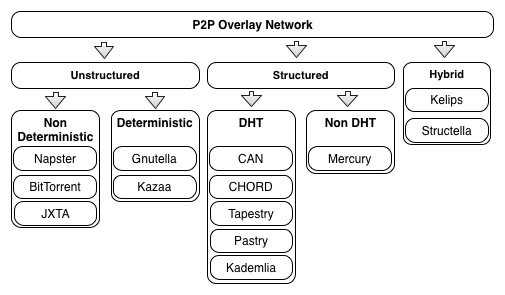
\includegraphics[width=\textwidth]{./img/p2porganizations.jpg}
  \end{center}
  \caption{Different types of P2P Overlay networks organizations}
  \label{fig:Different types of P2P Overlay networks organizations}
\end{figure}


\paragraph{\textbf{Unstructured -}} % (fold)
\label{par:Unstructured}

We call `Unstructured' to a P2P system that doesn't require or define any constraint for the placement of data, these include Napster, Kazaa and Gnutella, famous for it's file sharing capabilities, where nodes can share their local files directly, without storing the file in any specific Node. There is however a `caveat' in the Unstructured networks, by not having an inherent way of indexing the data present in the network, performing a lookup results of the cost of asking several nodes the whereabouts of a specific file or chunk of the file, creating a huge performance impact with an increasing number of nodes. In order to overcome this, Unstructured P2P networks offer several degrees of decentralization, one example is the evolution from Gnutella 0.4\cite{Definition2003} to Gnutella 0.6 \cite{T.Klingberg2002}\cite{Ripeanu2002a}, which added the concept of super nodes, entities responsible for storing the lookup tables for the files in parts of the network they are responsible for, increasing the performance, but adding centralized, single points of failure. 
\cite{Ranjan2006} classifies Unstructured networks into two types: deterministic and non-deterministic, defining that in a deterministic system, we can calculate before hand the number of hops needed to perform a lookup, knowing the predefined bounds, this includes systems such as Napster and BitTorrent\cite{Cohen2009}, in which the file transfers are decentralized, the object lookup remains centralized, keeping the data for the lookup tables stored in one place, which can be gathered by one of two ways : (i) peers inform directly the index server the files they have; or (ii) the index server performs a crawling in the network, just like a common web search engine, this gives this network a complexity of O(1) to perform a search, however systems like Gnutella 0.6, which added the super node concept, remain non deterministic because it's required to execute a query flood across all the super nodes to perform the search.

% paragraph Unstructured and Non-Deterministic (end)

\paragraph{\textbf{Structured with Distributed Hash Tables -}} % (fold)
\label{par:Structured with Distributed Hash Tables}

Structured P2P networks have an implicit way of allocating nodes for files and replicas storage, without the need of having any specie of centralized system for indexing, this is done by taking the properties of a cryptographic hash function \cite{Bakhtiari}\cite{Kargerl}\cite{Preneel1999}, such as SHA-1\cite{D.Eastlake3rdMotorola;P.JonesSystems2001}, which applies a transformation to any set of data with a uniform distribution of possibilities, creating an index with O(log(n)) peers, where the hash of the file represents the key and gives a reference to the position of the file in the network.
DHT's such as Chord\cite{Stoica2001}, Pastry\cite{Rowstron2001} and Tapestry\cite{Zhao2001}, use a similar strategy, mapping the nodes present in the network inside an hash ring, where each node becomes responsible for a segment of the hash ring, leveraging the responsibility to forward messages across the ring to his `fingers'(nodes that it knows the whereabouts). Kademlia\cite{Maymounkov} organizes it's nodes in a balanced binary tree, using XOR as a metric to perform the searches, while CAN\cite{Handley} introduced and a several dimension indexing system, in which a new node joining the network, will split the space with another node that has the most to leverage.
Evaluating the DHT Structured P2P networks raises identifiable issues/challenges, that result as the trade-off of not having an centralized infrastructure, responsible for railing new nodes or storing the meta-data, these are: (i) generation of unique node-ids is not easy achievable, we need always to verify that the node-id generated doesn't exist, in order to avoid collisions; (ii) the routing table is partitioned across the nodes, increasing the lookup time as it scales.
Table \ref{table:Complexity of structured P2P systems using a DHT}, showcases a comparison of the studied DHT algorithms.

\begin{table}
  \begin{tabular}{| p{1.4cm} | p{1.9cm} | p{2cm} | p{2.5cm} | p{1.6cm} | p{1.8cm} | p{1.8cm} |}
    \hline                        
    \textbf{P2P system} & \textbf{Overlay Structure} & \textbf{Lookup Protocol} & \textbf{Networking parameter} & \textbf{Routing table size} & \textbf{Ruting complexity} & \textbf{Join/leave overhead} \\
    
    \hline
    Chord & 1 dimension, Hash ring & Matching key and NodeID & n= number of nodes in the network & O(log(n)) & O(log(n)) & O(log(n)\textsuperscript{2}) \\
    
    \hline
    Pastry & Plaxton style mesh structure & Matching key and prefix in NodeID & n\= number of nodes in the network, b\=base of identifier & O(log\textsubscript{b} (n)) & O(b log \textsubscript{b} (n)+b) & O(log(n)) \\
    
    \hline
    CAN & d-dimensional ID Space & Key value pair map to a point P in the D-dimensional space & n= number of nodes in the network, d=number of dimensions & O(2d) & O(d n\textsuperscript{1/2}) & O(2d) \\
    
    \hline
    Tapestry & Plaxton style mesh structure & Matching suffix in NodeID & n=number of nodes in the network, b=base of the identifier & O(log\textsubscript{b}(n)) & O(b log \textsubscript{b} (n)+b) & O(log(n)) \\
    
    \hline  
    Kademlia & 2 & 3 & 4 & 5 & 6 & 7 \\
    \hline      
  \end{tabular}
  \caption{Summary of complexity of structured P2P systems}
  \label{table:Complexity of structured P2P systems using a DHT}
\end{table}

% paragraph Structured with Distributed Hash Tables (end)

\paragraph{\textbf{Structured without Non-Distributed Hash Tables -}} % (fold)
\label{par:Structured without Non-Distributed Hash Tables}

Mercury\cite{Bharambe}, a structured P2P network that uses a non DHT model, was design to enable range queries over several attributes that data can be dimensioned on, which is desired on searches over keywords in several documents of text. Mercury design offers an explicit load balancing without the use of cryptographic hash functions, organizing the data in a circular way, named `attribute hubs'.

% paragraph Structured without Non-Distributed Hash Tables (end)

% \paragraph{\textbf{Hybrid -}} % (fold)
% \label{par:Hybrid}
%TODO Structella , Kelips


% In recent developments, new generation P2P systems have evolved to combine both unstructured and structured P2P networks. We refer to this class of systems as hybrid. Structella [27] is one such P2P system that replaces the random graph model of an unstructured overlay (Gnutella) with a structured overlay, while still adopting the search and content placement mechanism of unstructured overlays to support complex queries. Other hybrid P2P design includes Kelips [60] and its variants. Nodes in Kelips overlay periodically gossip to discover new members of the network, and during this process nodes may also learn about other nodes as a result of lookup
% 12
% communication. Other variant of Kelips [56] allows routing table entries to store information for every other node in the system. However, this approach is based on assumption that system experiences low churn rate [70]. Gossiping and one-hop routing approach has been used for maintaining the routing overlay in the work [108]. In Table 4, we summarize the different P2P routing substrate that are utilized by the existing algorithms for organizing a GRIS.


% paragraph Hybrid (end)



\subsubsection{3.2.4 Fault Tolerance, Assurance and Trust}

Volunteer resource sharing means that we no longer have our computational infrastructure in a confined and very well monitored place, introducing new challenges that we have to address \cite{Koloniari2005} to maintain the system running with the minimum service quality, this issues can be: scalability, fault tolerance and security\cite{Wallach} of the data and that the system doesn't get compromised. This part of the document serves to describe the techniques implemented in previous non centralized systems to address this issues.

\paragraph{Fault Tolerance} % (fold)
\label{par:Fault Tolerance}
%TODO PAST + FUSE 





% paragraph Fault Tolerance (end)

\paragraph{Assurance and Trust} % (fold)
\label{par:Assurance and Trust}
%TODO Threshold Cryptography
%TODO Reputation Management
%TODO Economic Models




% paragraph Assurance and Trust (end)





% 
%---------{Resource sharing using the Web as platform}------------
% 
\subsection{Resource sharing using the Web as platform} 
%TODO Changed in the web Platform


\subsubsection{3.3.X What has been happening}
%TODO Javascript
%TODO WebRTC
%TODO HTTP 2.0
%TODO Banana bread

\subsubsection{3.3.X Previous attempts}
%TODO Merelo and friends





% ^^^^^^^^^^^^^^^^^^^^^^^^^^^^^^^^^^^^^^^^^^^^^^^^^^^^^^^^^^^^^^
% ~~~~~~~~~~~~~~~~~~~~~~~~~~~~~~~~~~~~~~~~~~~~~~~~~~~~~~~~~~~~~~
% ______________________________________________________________

% 
% Architecture
% 

\section{Architecture}
%TODO 


\subsection{Node Level}
%TODO 

\subsection{Client API}
%TODO 

\subsection{Storage}
%TODO 

\subsection{Reputation Mechanism}
%TODO 

\subsection{Job Scheduling}
%TODO 



% ^^^^^^^^^^^^^^^^^^^^^^^^^^^^^^^^^^^^^^^^^^^^^^^^^^^^^^^^^^^^^^
% ~~~~~~~~~~~~~~~~~~~~~~~~~~~~~~~~~~~~~~~~~~~~~~~~~~~~~~~~~~~~~~
% ______________________________________________________________

% 
% Evaluation
% 

\section{Evaluation}
%TODO 

\subsection{Lorem ipsum}
%TODO 

\subsubsection{Excepteur sint}
%TODO 


% ^^^^^^^^^^^^^^^^^^^^^^^^^^^^^^^^^^^^^^^^^^^^^^^^^^^^^^^^^^^^^^
% ~~~~~~~~~~~~~~~~~~~~~~~~~~~~~~~~~~~~~~~~~~~~~~~~~~~~~~~~~~~~~~
% ______________________________________________________________

% 
% Conclusions
% 

\section{Conclusions}
%TODO 

\subsection{Lorem ipsum}
%TODO 

\subsubsection{Excepteur sint}
%TODO 








% ^^^^^^^^^^^^^^^^^^^^^^^^^^^^^^^^^^^^^^^^^^^^^^^^^^^^^^^^^^^^^^
% ~~~~~~~~~~~~~~~~~~~~~~~~~~~~~~~~~~~~~~~~~~~~~~~~~~~~~~~~~~~~~~
% ______________________________________________________________


% 
% Acronym List
% 

% \acro{abc}[short version]{full version}
% \acro{efd}[shortAAA version]{full AAAversion}


% ^^^^^^^^^^^^^^^^^^^^^^^^^^^^^^^^^^^^^^^^^^^^^^^^^^^^^^^^^^^^^^
% ~~~~~~~~~~~~~~~~~~~~~~~~~~~~~~~~~~~~~~~~~~~~~~~~~~~~~~~~~~~~~~
% ______________________________________________________________

% 
% Bibliography
% 

\bibliographystyle{plain} 
\bibliography{/Users/DavidDias/Documents/bibtex/THESISREAD.bib}
\end{document}